%!TEX root = UG_PhD_Defense.tex
%Single-fix Rectification
%Show our current progress on single fix rectification
%redundancy?

% \begin{frame}{\large Single-fix Rectification: Prior work}
% \bi
% 	\item Automated Diagnosis: Boolean Reasoning [{\it Madre. et al}, ICCAD'89] [{\it Liaw. et al}, ICCAD'90]
% 	\item Engineering Change Order (ECO): CNF-SAT formulation
%  	[{\it Marek-Sadowska. et al}, DAC'95] [{\it Huang. et al}, ICCAD'10] 
%  	\item Partial Synthesis: Quantified Boolean Formula(QBF)
%  	[{\it Scholl. et al}, ICCD'13] [{\it Fujita. et al}, Proc IEEE'15]
%  	\item Symbolic Computer Algebra techniques:
%  	\bi
%  		\item Rectification of finite field circuits [{\it Rao. et al}, FMCAD'18][{\it Gupta. et al}, VLSI-SOC'18]
%  		\item  Automated Debugging of integer arithmetic circuits using Computer Algebra
% 			[{\it Mishra. et al}, ICCD'17] [{\it Mishra. et al}, DATE'16] [{\it Ciesielski. et al}, DAC'15]
% 			% \bi
% 			% \item Incorrect and incomplete: Approach heavily relies on the structure of the circuit
% 			% \ei
%  	\ei
% \ei
% \end{frame}

\begin{frame}{\large Application: Single-Fix Rectification}
\bi
	\item Circuit designed over $\Fkn = \F_{2^2} (n=2)$ using irreducible polynomial $P_n(x) = P_2(x) = x^2+x+1$ with $P_2(\ga)=0$
\ei
\begin{figure}[hbt]
    \begin{center}
    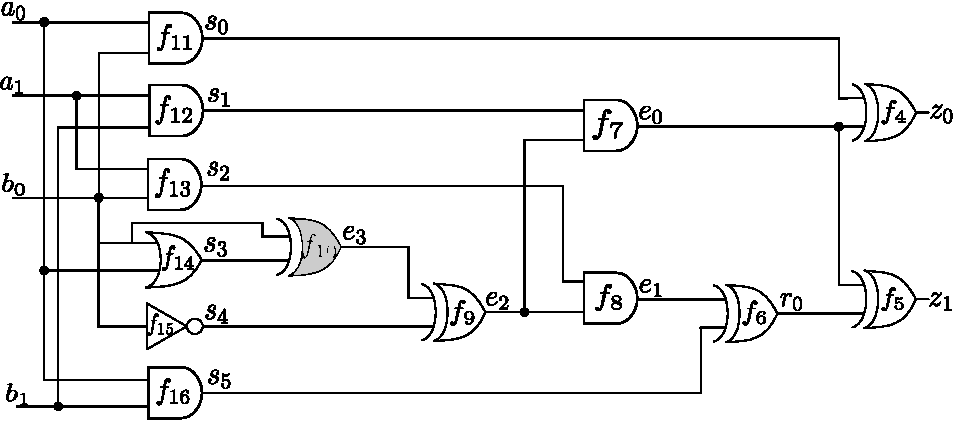
\includegraphics[scale = 0.64]{mas_red_bug-eps-converted-to.pdf}
    \end{center}
%    \vspace{-4ex}
    \caption*{\small A 2-bit faulty modulo
      multiplier implementation. 
    %   with the bug at
    % net $e_3$. A correct implementation will have an AND gate at $e_3$,
    % which has been replaced by an XOR gate.
    }
    \label{fig:mas_both}
\end{figure}

\end{frame}

\begin{frame}{\large SFR Application: Verification}
\bi
	\item Denote polynomial $f: Z + A\cdot B$ as the design specification.
	\item Impose RTTO $>$
\ei
\[ \begin{array}{lll}%									   
f_1:Z + z_0 +\ga \cdot z_1;&\quad  f_7:e_0 + s_1e_2; 	   &\quad f_{12}:s_1 + a_1b_1; \\
f_2:A + a_0 +\ga \cdot a_1;&\quad  f_8:e_1 + s_2e_2; 	   &\quad f_{13}:s_2 + a_1b_0;  \\
f_3:B + b_0 +\ga \cdot b_1;&\quad  f_9:e_2 + e_3 + s_4;    &\quad f_{14}:s_3 + a_0 + b_0 + a_0b_0; \\ 
f_4:z_0 + s_0 + e_0;  	   &\quad  \alert{f_{10}:e_3 + b_0 + s_3;} &\quad f_{15}:s_4 + b_0 + 1;\\ 
f_5:z_1 + e_0 + r_0;  	   &\quad  f_{11}:s_0 + a_0b_0;    &\quad f_{16}:s_5 + a_0b_1;  \\
f_6:r_0 + e_1 + s_5;            						    
\end{array}\]%

\bi
	\item $F = \{f_1,\dots,f_{16}\}$, $F_0 = \{a_0^2-a_0, a_1^2-a_1,
b_0^2-b_0, b_1^2-b_1\}$
	\item Ideal Membership Test: $f\xrightarrow{F,F_0}_+\ga^1\cdot (a_0a_1b_1b_0+a_0a_1b_1+a_1b_1b_0+a_1b_0) + \ga^0\cdot (a_0a_1b_1b_0+a_0a_1b_1+a_1b_1b_0)$
\ei
\end{frame}

% \begin{frame}{\large Application: Single-Fix Rectification}
% \bi
% 	\item Circuit designed over $\Fkn$ using irreducible polynomial $P_n(x) = P_2(x) = x^2+x+1$ with $P_2(\ga)=0$
% \ei
% \begin{figure}[hbt]
%     \begin{center}
%     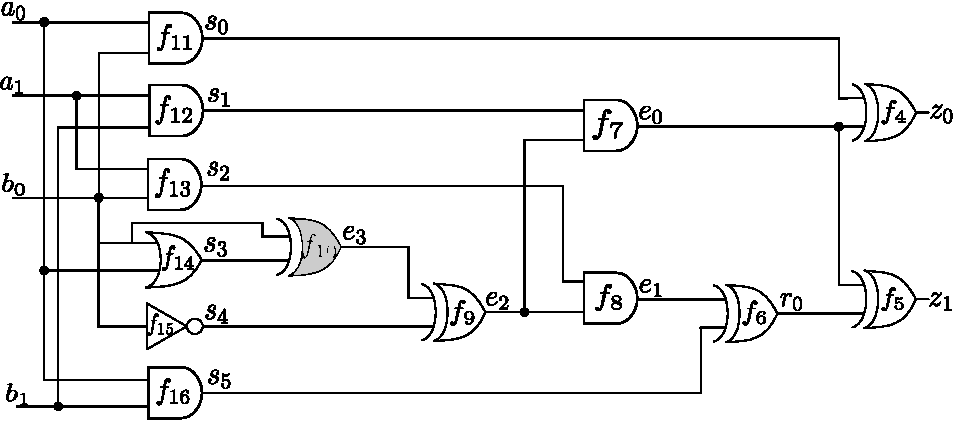
\includegraphics[scale = 0.64]{mas_red_bug-eps-converted-to.pdf}
%     \end{center}
% %    \vspace{-4ex}
%     \caption*{\small A 2-bit buggy modulo
%       multiplier implementation. 
%     %   with the bug at
%     % net $e_3$. A correct implementation will have an AND gate at $e_3$,
%     % which has been replaced by an XOR gate.
%     }
%     \label{fig:mas_both}
% \end{figure}

% \end{frame}

% \begin{frame}{\large SFR Contribution: Identifying Target Nets}
% %We are investigating; and we have some ideas; I will tell you what it is
% %We use a specific order (start from PO); Compute GB with this order; 
% %LEX order eliminates vars; what ends up happening is we get a set of poly
% % in PI and analyze those polynomials; no need to simulation 
% % It's a conjecture that I am targeting; we believe me can formally prove it
% %Suppose we find it; then intersection of cones(figure)
% % Rudimentary approach: If the bug  is observable at multiple outputs, then
% % single-fix rectification is possible at one of the nets 
% % Once GB is computed, the structure of GB is such that
% % we will find exactly one polynomial of the form $t(P)+1$.
% % $P$  

% \begin{figure}
% \centering
% 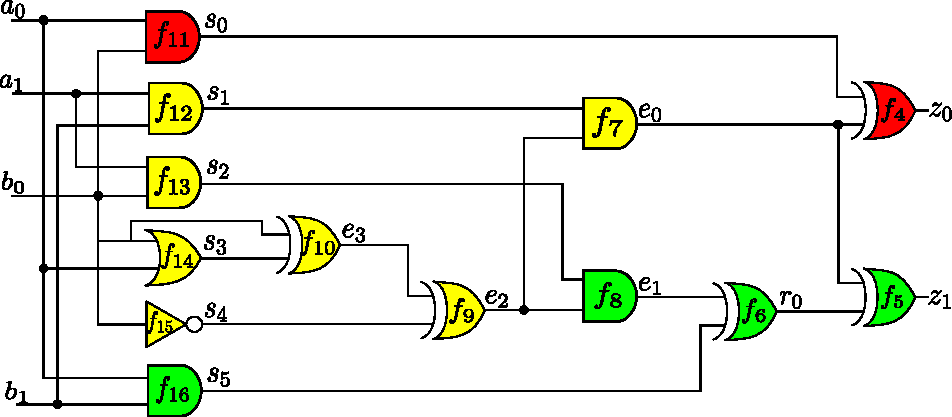
\includegraphics[scale=0.58]{mas_2_bugs_cones.pdf}
% \end{figure}
% \bi
% 	\item Set of affected outputs: $\Oa = \{z_0,z_1\}$
% 	\item Intersection of set of nets in fan-in cones of $\Oa$: $\mN = \{s_4,s_3,s_2,s_1,e_3,e_2,e_0\}$
% 	\item Single-Fix rectification can only exist at a net $x_i \in \mN$
% 	% \item Currently under investigation
% 	% \item Use a specific term order for writing the polynomials
% 	% \item Due to this term-order, GB performs elimination
% 	% \item Analyze polynomials in PI to list POs where error observable
% \ei

% \end{frame}


\begin{frame}{\large SFR Application: Rectification Check}
%ATPG V() V() = empty
%we have an algebraic proof which is there in the proposal
% \bi
	% \item Single-fix rectification exists at net $x_i$, {\it iff} $V_{\Fq}(r_L) \cup V_{\Fq}(r_H) =
 % 		\Fq^{|X_{PI}|} = V(J_0^{PI}) $
	\vspace{0.1in}
	% Single-fix patch modeled over $\Fkm = \F_{2} (m=1)$ within a circuit 
	% modeled over $\Fkn = \F_{2^2}$
	\begin{enumerate}
		\item Rectification check at net $e_3$: $W = \{e_3\}$
		\bi
			\item $J_1 = \langle F_1\rangle$, where $F_1=\{f_1,\dots, f_{10}=e_3+0,\dots, f_{16}\}$
			\item $J_2 = \langle F_2\rangle$, where $F_2 = \{f_1,\dots, f_{10}=e_3+1,\dots, f_{16}\}$
		\ei
		\vspace{0.1in}
		\item Compute $r_1$ and $r_2$:
		\bi
			\item $r_1 = f \xrightarrow[]{J_1, J_0}_+{(\ga+1)a_1b_1b_0+(\ga+1)a_1b_1}$
			\item $r_2 = f \xrightarrow[]{J_2,J_0}_+{(\ga+1)a_1b_1b_0+(\ga)a_1b_0}$
		\ei
		\vspace{0.1in}
		% \item Single-fix rectification possible iff $G = GB(r1\cdot r2, F_0)=F_0$
		\item Single-fix rectification possible iff $V(r_1) \cup V(r_2) = \F_{2^3}^{|X_{PI}|} = V(J_0)$
		\bi
			\item Compute $G = GB(r1\cdot r2, J_0)$ and check if $G=J_0$
			\item In this example, target $e_3$ admits SFR
		\ei
	\end{enumerate}
% \ei
\end{frame}

% \begin{frame}{\large SFR Application: Computing Rectification Function}
% \bi
% 	\item Rectification check confirmed there exists a polynomial at net $e_3$: $f_{10}: e_3 + U$ that can
% 	rectify the circuit. 
% 	\bi
% 		\item Here $U$ is the \textit{unknown component} to be computed.
% 	\ei
% 	\item Update $F$ to $F=\{f_1,\dots,f_{10} = e_3+U,\dots,f_{16}\}$
% 	\item For a correct implementation, $f\xrightarrow{F\cup F_{0}^{PI}}_+0$ still holds
% 	\item Obtain the remainder $r$ and quotient of division $h_{10}$ as:
% 	\bi
% 		\item $f\xrightarrow[]{{f_1}}\dots\xrightarrow[]{{e_3}}[\underbrace{{(\ga+1)s_1+\ga s_2}}_\text{$h_{10}$}]({e_3})+\{\underbrace{{\scriptstyle s_0+(\ga+1)s_1s_4+\ga s_2s_4+\ga s_5+\ga a_0b_1+a_0b_0+(\ga+1)a_1b_1+\ga a_1b_0\}}}_\text{$r$}$
% 	\ei
% 	\item The \textit{unknown component} problem is then formulated as an ideal membership test and
% 	solved using extended \Grobner Basis: 
% 	\bi
% 		\item $r \in \langle h_{10},f_{11},f_{12},f_{13},f_{14},f_{15},f_{16}\rangle
% 	  		+ \langle F_{0}^{PI}\rangle$.
% 		\item $U=b_0$, i.e. $f_{10} = e_3 + b_0$
% 	\ei
% \ei
% \end{frame}

\begin{frame}{\large Unified framework motivation}
\bi
	\item Single-fix is a special case of MFR with $m=1$
	\bi
		\item Rectification patch modeled over $\Fkm = \F_{2^1} = \F_2$
		\item Circuit modeled over $\Fkn$ 
		\bi
		    \item Since $m=1$ divides $n$, $\F_2 \subset \F_{2^n}$, $\forall n \in \Z_{>1}$
		\ei
	\ei
	\vspace{0.1in}
	\item For Multi-fix, since $m > 1$, $\Fkm$ might not be contained in $\Fkn$
	\bi
		\item Ex. $\F_{2^2}$ is not contained in $\F_{2^3}$, $m=2,n=3$
	\ei  
	\vspace{0.1in}
	\item Need a higher composite field $\Fkk$ such that 
	\bi
		\item $\Fkm \subset \Fkk$ and $\Fkn \subset \Fkk$
	\item What are the mathematical challenges?
	\item What primitive polynomial $P_K(x)$ should be used for constructing $\Fkk$
	\ei
\ei
\end{frame}